\subsection{Results}
\label{thresholdresults}
{\color{black}To understand the appropriate balance of migrating pages early (as soon as first touch on the GPU) or later (when partial information about page hotness is known),
we implemented a page migration policy in which pages become candidates for software controlled page migration only after they are touched
$N$ times by the GPU\@. Strictly migrating pages on-demand before servicing the memory requests will put 
page migration on the critical path for memory load latency. However, migrating a page after
$N$ references reduces the number of accesses that can be serviced from the GPU local memory, decreasing the potential
impact of page migration.} Once a page crosses the threshold for migration, we place it in an unbounded FIFO queue for migration, and allow
the CUDA software runtime to migrate the pages by polling this FIFO and migrating pages as described
in the previous sub-section.  

To isolate the effect of choosing a threshold value from TLB shootdown costs, we optimistically assume a TLB shootdown 
and refill overhead of 0 cycles for the results shown in Figure~\ref{fig:threshold}. This figure shows application
performance when migrating pages only after they have been touched $N$ times,
represented as threshold-$N$ in the figure.   The baseline
performance of 1.0 reflects application performance if the GPU only accesses the CPU's DDR via hardware cache coherence and no page migrations
to GDDR occur.  Although we anticipated using a moderately high threshold (64--128) would generate the best performance
(by achieving some level of differentiation between hot and cold data), the results in the figure indicate that, for the majority of the benchmarks, using the lowest threshold 
typically generates the best performance.  Nevertheless, behavior and sensitivity to the threshold varies significantly across applications.

\begin{figure}[t]
    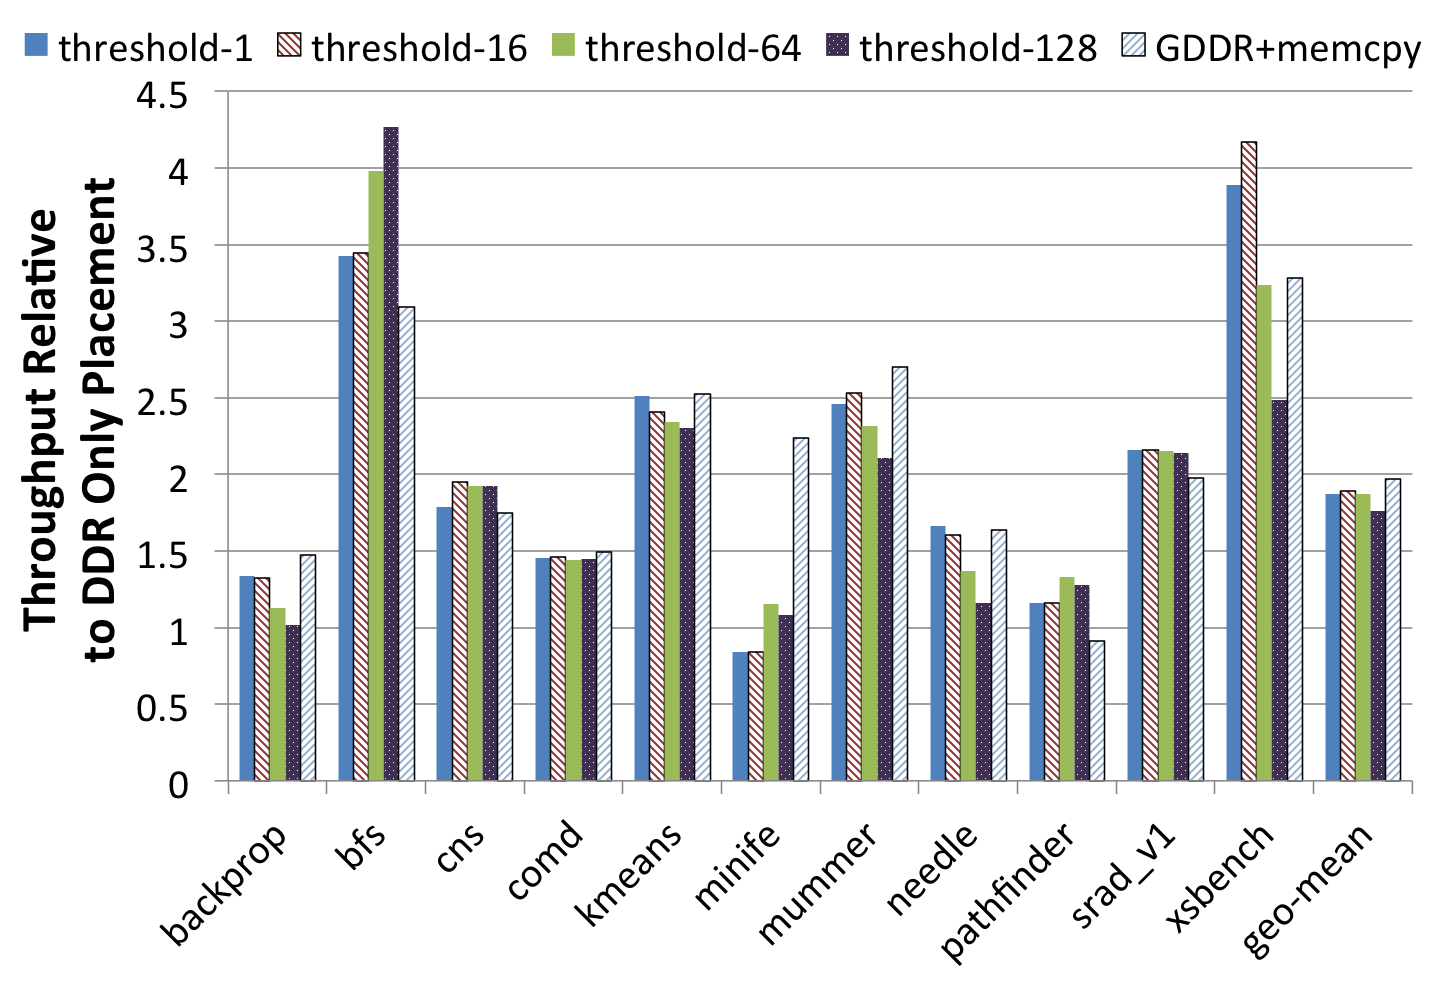
\includegraphics[width=\columnwidth]{hpca2015/figures/staticthreshold.png} 
    \caption{Performance of applications across varying migration thresholds, where threshold-N is the number of touches a given page must receive
    before being migrated from CPU-local to GPU-local memory.}
    \label{fig:threshold}
\end{figure}

For the majority of our workloads, the best performance comes at a low migration threshold
with performance degrading as the threshold increases.  The peak performance is well above that achievable with 
only cache-coherent access to DDR memory, but it rarely exceeds the the
performance of the legacy {\tt memcpy} programming
practice. The {\tt bfs} benchmark is a notable outlier, with higher migration thresholds improving performance by successfully differentiating hot
and cold pages as candidates for migration.  However, performance variation due to
optimal threshold selection is much smaller than the substantial performance gain of using any migration policy.  {\tt Minife}
is the second substantial outlier, with a low migration threshold decreasing performance below that of using CPU-only
memory, while migration with higher thresholds provides only modest gains over  cache-coherent access to DDR\@. Further analysis revealed 
that, for this workload, migration often occurs after the application has already performed the bulk of its accesses to a given
page.  In this situation, page migration merely introduces a bandwidth tax on the memory subsystem with little possibility for
performance gain.  

To implement a threshold-based migration system in practice requires tracking the number of times a given physical page
has been touched.  Such counting potentially requires tracking all possible physical memory locations that the GPU may access
and storing this side-band information either in on-chip SRAMs at the L2, memory controller, or within the DRAM itself.  Additional
coordination of this information may be required between the structures chosen to track this page-touch information. Conversely,
a first touch policy (threshold-1) requires no tracking information and can be trivially implemented by migrating a page the first time
the GPU translates an address for the page.  Considering the performance differential
seen across thresholds, we believe the overhead of implementing the necessary hardware counters to track all pages within a system 
to differentiate their access counts is not worth the improvement over a vastly simpler first-touch migration policy.

In Figure~\ref{fig:threshold} we showed the performance improvement achievable 
when modeling the bandwidth cost of the page migration while ignoring the 
cost of the TLB shootdown, which will stall the entire GPU.  At low migration 
thresholds, the total number of pages migrated is largest and thus application 
performance is most sensitive to the overhead of the TLB shootdown and refill. 
Figure~\ref{fig:migrationoverheads} shows the sensitivity of application 
slowdown to the assumed cost of GPU TLB shootdowns for a range of client-side 
costs similar 
to those investigated by Villavieja et al.~\cite{Villavieja2011}. 
While the TLB invalidation cost in current GPUs is much higher, due to complex 
host CPU interactions, it is likely that TLB invalidation cost will drop 
substantially in the near future (due to IOMMU innovation) to a range 
competitive with contemporary CPUs (i.e., ~100 clock cycles).

Because the GPU comprises many concurrently executing pipelines, the performance 
overhead of a TLB shootdown, which may require flushing all compute pipelines, is 
high; it may stalls thousands of execution lanes rather than a single CPU core.  
Figure~\ref{fig:migrationoverheads} shows that moving from an idealized threshold of 
zero, to a realistic cost of one hundred reduces average performance by 16\%.  In 
some cases this overhead can negate the entire performance improvement achieved 
through page migration. To maximize the performance under page migration, our 
migration mechanism must optimize the trade-off between stalling the GPU on TLB 
shootdowns versus the improved memory efficiency of migrating pages to the GPU\@.  
One way to reduce this cost is to simply perform fewer page migrations, which can 
be achieved by increasing the migration threshold above the 
migrate-on-first-touch policy.  Unfortunately, a higher migration threshold also 
decreases the potential benefits of migration.  Instead, we will describe 
mechanisms that can reduce the number of required TLB invalidations simply 
through intelligent page selection while maintaining the first-touch 
migration threshold.

\begin{figure}[t]
    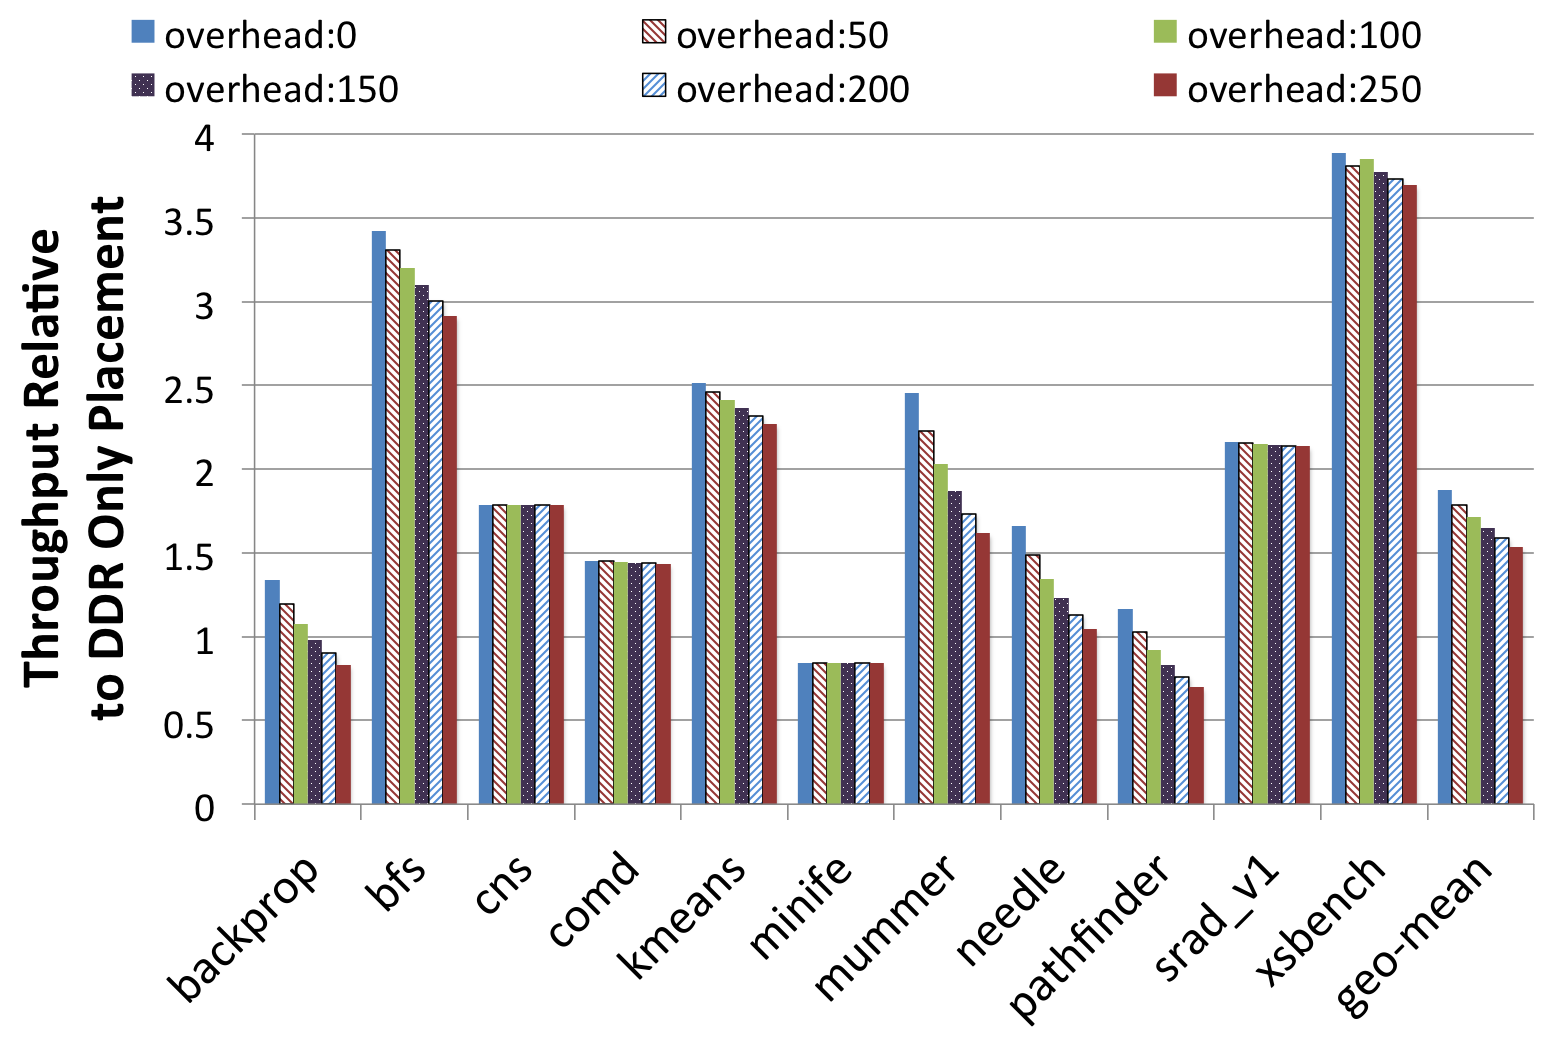
\includegraphics[width=\columnwidth]{hpca2015/figures/migrationoverheads.png} 
    \caption{Performance overhead of GPU execution stall due to TLB shootdowns when using a first touch migration policy (threshold-1).}
    \label{fig:migrationoverheads}
\end{figure}
